% !TEX root = ../main.tex

\chapter{多卡并行扩展与归并优化}

\section{多卡扩展需求分析}

第四章已经从单 GPU 视角完成了系统级优化，并初步说明在 GPU 主导端到端执行链路、异步 I/O---计算流水线和后端重构协同作用下，单卡场景中的主要损耗从主机---设备边界转向设备侧检索与评分过程。随着输入规模继续增大、查询并发进一步提升、候选索引逼近单卡显存上限，单卡系统仍会同时遭遇三类上限：计算上限、容量上限和调度上限。

第一类需求来自计算上限。当候选召回和异常评分都已稳定驻留在 GPU 侧时，单卡吞吐最终会受限于单设备的计算资源。此时，即便继续压缩局部路径开销，系统整体 QPS 仍然难以随业务峰值线性提升。第二类需求来自显存与索引容量上限。在更大索引或更大规模合成扩展数据集条件下，单 GPU 可能无法同时容纳完整索引、副本缓存以及评分中间张量，系统必须在缩小索引规模、降低候选预算和增加设备数量之间进行权衡\citep{cuvs_multi_gpu_nn,cuvs_multi_gpu_ivf_host}。第三类需求则来自调度压力。金融近实时异常检测同时要求平均吞吐、延迟分位数和资源利用率保持稳定；一旦请求在单设备上集中堆积，即使平均性能尚可，尾延迟也会迅速恶化。

因此，对本文系统而言，多 GPU 扩展需要在保持检测效果、延迟分位数和实现复杂度可控的前提下解决三个问题：如何把更多查询稳定分摊到多张 GPU 上，如何在容量受限时继续维持索引可用性，以及如何避免调度与共享路径重新成为系统上限\citep{cuvs_multi_gpu_nn}。进入多卡场景后，局部结果如何归并、CPU 是否重新回到关键路径、共享存储路径是否发生拥塞，都会直接影响扩展收益能否兑现。

基于这一判断，本文后续优先采用索引复制（replicated）架构主方案，使每张 GPU 尽可能独立完成候选召回与异常评分；只有在索引容量或业务约束明确表明无法复制完整索引时，才进入设备侧跨卡归并与设备间通信的兜底路径。换言之，本章的关注点是在金融近实时异常检测场景下找到更符合吞吐优先和工程可控性的扩展方式，避免发散到构造复杂的多 GPU 检索系统。

\section{多卡扩展策略设计原则}

多 GPU 扩展方案的设计必须建立在系统目标与瓶颈分析的基础上。结合第四章单卡结论与第二章相关工作梳理，本文将多 GPU 扩展方案归纳为四项基本原则：查询级并行优于单查询跨卡并行；数据并行与索引复制优先于直接采用索引分片；CPU 保持在控制面；当跨卡归并不可避免时，优先采用 GPU 侧归并。前两项决定主方案形态，后两项约束兜底路径和运行边界。

首先，查询级并行优于单查询跨卡并行。若一个查询必须在多张 GPU 上分别完成局部搜索并在末端归并，系统会额外承担局部结果表达、跨卡通信和同步等待等成本；而当不同查询被均衡分发到不同 GPU 时，每张设备就更容易复用单卡阶段已经压缩好的``候选召回---异常评分''闭环。cuVS 多 GPU 文档将索引复制（replicated）模式描述为通过在各 GPU 间分发查询以获得更高查询吞吐（query throughput），这一点与本文的吞吐目标一致\citep{cuvs_multi_gpu_nn}。

在此前提下，第二项原则进一步限定了主方案选择：数据并行与索引复制优先于一开始即采用索引分片。cuVS 的分布模式定义表明，索引复制（replicated）更偏向吞吐优先，分片（sharded）更偏向容量扩展\citep{cuvs_multi_gpu_nn,cuvs_dist_mode}。因此，只要索引仍可复制，完整副本在每张 GPU 上独立服务本地查询，通常比从一开始就引入跨卡依赖更符合本文的系统目标。

第三项原则主要约束控制边界，即 CPU 保持在控制面而不重新回到结果处理主路径。cuVS 文档提示，多 GPU ANN 的部分实现要求数据集、查询与输出数组位于主机内存（host memory），这意味着若直接沿用主机中心式（host-centric）默认路径，则 CPU 与主机内存会重新进入关键路径\citep{cuvs_multi_gpu_ivf_host}。基于这一认识，本文在多 GPU 方案中将 CPU 定位为控制面调度者：它负责请求队列管理、负载均衡、有界批处理（bounded batching）、运行时监控和最终小规模结果汇总，但不承担大规模候选集合或评分中间张量的重新组织。

最后一项原则只在主方案不能直接成立时才发挥作用，即当必须跨卡归并时，归并逻辑尽量下沉到 GPU 侧，并通过 NCCL 等设备间通信机制完成。NCCL 文档指出其通信操作会异步入队到 CUDA stream 上执行，但也警告在同一 \texttt{ncclGroupStart/End()} 中混用多个 stream 会形成全局同步点\citep{nccl_stream_semantics}。GPU 侧归并优于 CPU 聚合，但仍然带来额外通信组织成本，因此本文将其明确为兜底路径。

表~\ref{tab:primary-vs-fallback} 对 FlashTOD 多 GPU 部署中的索引复制主方案、设备侧归并兜底路径以及主机侧聚合对比路径的适用边界进行了归纳。

\begin{table}[htbp]
  \caption{FlashTOD 多 GPU 部署适用边界}
  \label{tab:primary-vs-fallback}
  \centering
  \footnotesize
  \setlength{\tabcolsep}{2.6pt}
  \renewcommand{\arraystretch}{1.18}
  \begin{adjustbox}{max width=\linewidth}
    \begin{tabular}{P{2.4cm}P{3.1cm}P{3.2cm}P{3.0cm}P{2.8cm}}
      \toprule
      条件 & replicated 主方案 & 设备侧归并 & 主机侧聚合 & 主要风险 \\
      \midrule
      索引可完整复制，吞吐优先 &
      每卡保留完整索引，按查询或微批分发 &
      通常不需要启用，仅保留为容量受限兜底 &
      仅用于调试或小规模对照 &
      显存占用高，索引规模继续增大后可能失效 \\
      \midrule
      单卡无法容纳完整索引，需要容量扩展 &
      不再直接适用 &
      索引按卡分片，局部结果在 GPU 侧组织和归并 &
      可作为实现简单的对照路径 &
      跨卡通信、同步点和归并复杂度上升 \\
      \midrule
      原型验证、调试或离线分析 &
      可用于简化路径验证 &
      可与主机侧聚合形成对照 &
      各 GPU 输出局部结果后回传 CPU 排序合并 &
      CPU 重新进入数据平面，D2H/H2D 与排序开销放大 \\
      \bottomrule
    \end{tabular}
  \end{adjustbox}
\end{table}

该表用于说明不同多 GPU 路径的适用条件。本文当前结论限定在单机多 GPU、固定候选预算和固定硬件拓扑条件下：replicated 路径是吞吐优先主方案，设备侧归并是容量受限时的兜底路径，主机侧聚合主要用于形成可解释的对照基线。

\section{数据并行与索引复制的多卡执行架构}

基于前述设计原则，本文将多 GPU 场景下的主扩展方案定义为数据并行与索引复制（replicated）架构。索引复制架构适用于索引仍可在单张 GPU 显存内复制、查询吞吐优先且希望复用完整单卡链路的场景；该路径主要提升吞吐，不提升单卡可容纳的索引容量。这意味着，只要完整索引仍能复制到每张 GPU，本文就更倾向于用显存换取更简单的数据路径和更稳定的查询闭环\citep{cuvs_multi_gpu_nn}。在该方案中，完整索引被复制到每张 GPU 上，每张 GPU 都具备完整的候选召回与异常评分能力；查询按批次或微批次被分发到不同 GPU，各设备在本地独立执行``查询向量组织---候选召回---异常评分---局部结果输出''全链路流程；CPU 主要承担请求级调度、批次分配和最终小规模结果汇总职责。

在执行流程上，数据并行与索引复制架构可以形式化表示为：给定总查询集合 $Q=\{q_1,q_2,\ldots,q_m\}$，调度器将其划分为若干子批次 $\{B_1,B_2,\ldots,B_g\}$，并将这些子批次分配给 $g$ 张 GPU。每张 GPU $G_j$ 本地维护一份完整索引 $\mathcal{I}_j=\mathcal{I}$，对其收到的批次 $B_j$ 独立执行
\begin{equation}
  C_j = \mathcal{R}(B_j,\mathcal{I}_j), \qquad S_j = \mathcal{F}(B_j,C_j),
  \label{eq:multi-gpu-local-loop}
\end{equation}
式~\eqref{eq:multi-gpu-local-loop} 中，$\mathcal{R}$ 表示候选召回，$\mathcal{F}$ 表示异常评分。由于每张 GPU 都能本地完成完整闭环，因此系统不需要在查询处理中途引入设备间依赖。

从系统工程角度看，索引复制虽然会增加显存占用，但换来了更低的执行复杂度和更清晰的数据路径。其优势主要体现在三个方面：查询之间天然独立，便于按请求或微批次做吞吐扩展；每张 GPU 都能沿用第四章已经优化好的本地执行链路，不需要为多卡场景重新拆解候选召回与评分接口；系统只需在极小规模结果层面做收口，无需在处理过程中持续维护跨卡依赖。基于这些特点，本文将索引复制定义为多 GPU 扩展的主方案。

图~\ref{fig:replicated-arch} 给出了索引复制主方案的总体结构，直观展示了 CPU 控制面与 GPU 本地闭环在多卡场景下的分工关系。

\begin{figure}[!htbp]
  \centering
  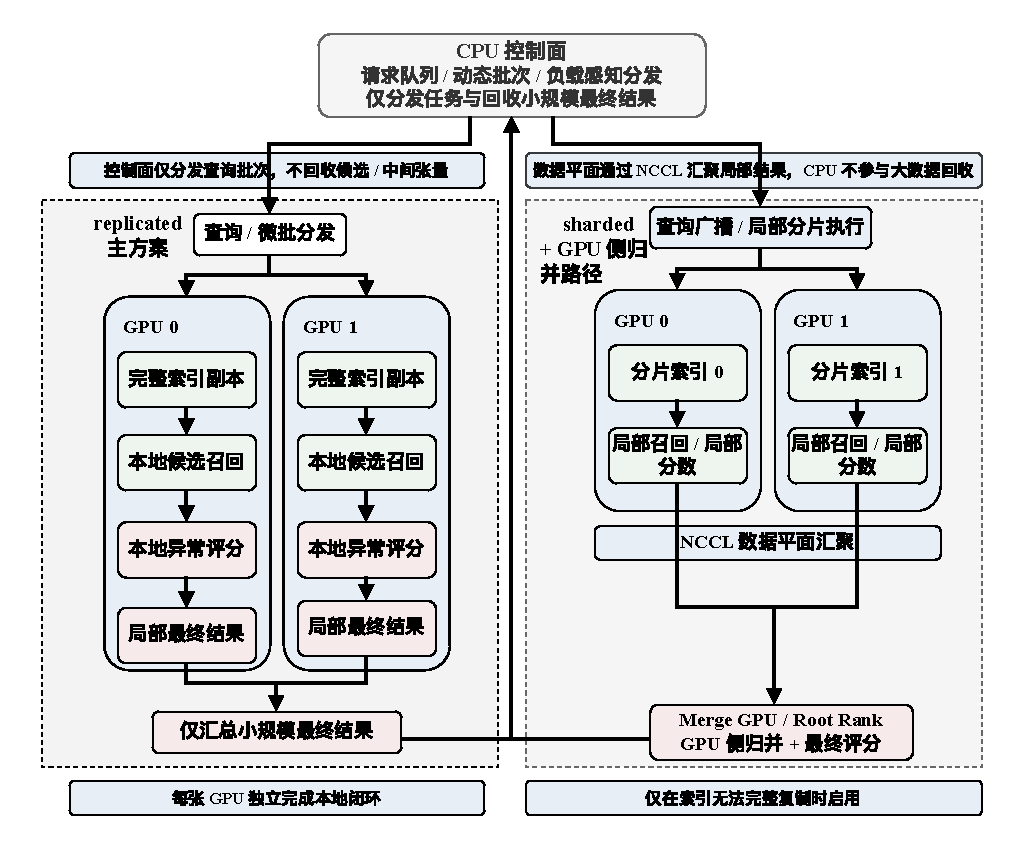
\includegraphics[width=\linewidth]{figures/fig5-1_multi_gpu_overall_architecture.pdf}
  \caption{数据并行与索引复制多 GPU 架构}
  \label{fig:replicated-arch}
\end{figure}

\section{CPU 控制面调度与负载均衡}

在索引复制（replicated）架构下，CPU 的职责需要被严格限定。本节所讨论的控制面工作主要包括请求队列维护、微批形成、按 GPU 负载分发批次、控制 bounded batching 策略，以及在各 GPU 完成本地闭环之后接收最终小规模输出。

请求队列组织方面，系统采用统一入口队列接收查询请求，并根据队列长度、GPU 空闲度和微批策略动态形成批次。低时延推理系统和可预测深度学习服务系统的研究都表明，面向吞吐与尾延迟的批处理策略，需要在设备利用率和排队时间之间做持续折中；cuVS 动态批处理文档则为本文的多 GPU 实现提供了更接近工程接口层的参考\citep{crankshaw2017clipper,gu2020clockwork,cuvs_dynamic_batching}。本文把微批作为调节吞吐和尾延迟的控制旋钮：批次过小会浪费设备并行能力，批次过大又会推高排队等待。

负载均衡方面，本文在索引复制架构下优先采用查询级动态调度而非静态平均分配。cuVS 在索引复制模式下提供了 \texttt{LOAD\_BALANCER} 与 \texttt{ROUND\_ROBIN} 两类搜索模式，其中前者用于保持各 GPU 负载均衡\citep{cuvs_dist_mode}。这类调度能够防止某张 GPU 因瞬时队列堆积而拉高整机的第 99 百分位延迟（p99 延迟），避免只在形式上平均分配请求。

最终结果汇总方面，CPU 仅接收每张 GPU 已完成的最终小规模结果，如异常分数、Top-$k$ 排序结果和必要日志元信息。局部候选集合、评分中间张量以及归并前的设备侧结构都不应回流到 CPU。

图~\ref{fig:control-plane} 展示了 CPU 控制面的调度与回收流程，控制面与数据平面的职责边界将在正文中结合各组件的关键参数分别说明。

\begin{figure}[!htbp]
  \centering
  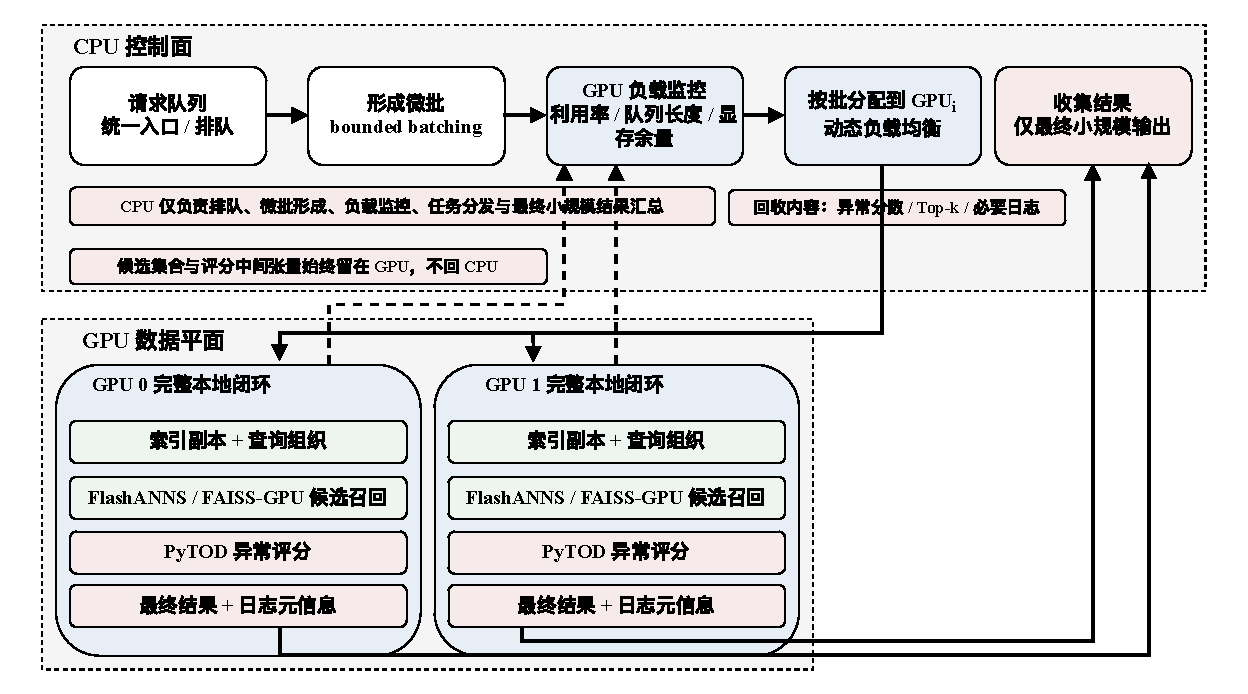
\includegraphics[width=\linewidth]{figures/fig5-2_cpu_control_plane_microbatch.pdf}
  \caption{CPU 控制面调度与微批示意}
  \label{fig:control-plane}
\end{figure}

图中 FAISS-GPU 表示前期候选召回接口验证路径；多 GPU 完整路径下的本地候选生成以后续接入的 FlashANNS 候选召回前端为主。

\section{跨卡归并场景下的 GPU 侧归并与 NCCL 通信}

当索引容量超过单卡显存可容纳范围，或业务约束要求单一查询必须访问分布在多张 GPU 上的局部索引时，索引复制主方案就不再直接适用，系统必须进入跨卡归并场景。本文把这一场景明确界定为兜底路径：只有在主方案因容量或部署条件失效时，才引入分片索引与跨卡结果合并。因为一旦进入归并路径，系统就必须额外承担局部结果表达、设备间通信和流协调等成本。

在此条件下，本文仍坚持一个约束：局部结果尽量在 GPU 侧组织与合并，CPU 只接收最终极小规模结果。cuVS 在分片模式下给出了 \texttt{MERGE\_ON\_ROOT\_RANK} 与 \texttt{TREE\_MERGE} 两类归并方式，为本文设计设备侧归并路径提供了参考\citep{cuvs_dist_mode}。与主机侧聚合路径相比，设备侧归并路径的主要收益在于减少大规模结果回传和主机侧排序开销，使跨卡合并尽可能延续设备侧处理逻辑；额外的通信与同步组织也使其复杂度高于索引复制主方案。

在设备间通信实现方面，本文采用 NCCL 作为主要通信机制，并将通信流与局部计算流明确分离。NCCL 文档指出其通信操作异步入队到指定 CUDA stream，但在同一 \texttt{ncclGroupStart/End()} 组内混用多个 stream 会形成全局同步点\citep{nccl_stream_semantics}。因此，GPU 侧归并的收益建立在一个前提上：通信必须被控制在必要范围内，并与本地计算流合理解耦。若通信组织不当，兜底方案很容易因同步点过多而侵蚀掉原本希望保留的扩展收益。

\section{拓扑感知 I/O 通道绑定与准入控制}

在多 GPU 异常检测系统中，扩展上限不仅由 GPU 数量决定，还受制于存储路径和 PCIe/NUMA 拓扑。单卡阶段被压缩掉的路径开销，在多卡环境下可能以另一种形式重新出现：如果多张 GPU 共享同一 SSD 通道或 PCIe 路径，局部检索和候选读取虽然仍在设备侧执行，但共享链路上的排队会直接反映到吞吐下降和 p99 延迟上升。GDS 概览文档指出，GDS 通过在 GPU 显存与存储设备之间建立直接内存访问（Direct Memory Access，DMA）路径来避免 CPU bounce buffer，并强调拓扑路径会影响传输效率\citep{gds_overview}。基于这一认识，本文引入拓扑感知 I/O 通道（I/O lane）绑定与准入控制机制：运行前分析 GPU、SSD、PCIe 根复合体（PCIe root complex）、PCIe 交换机（PCIe switch）与 NUMA 节点之间的关系；运行时尽量将 GPU 与 SSD 通道进行绑定，并对每条 I/O 通道的在途请求（in-flight requests）数做有界控制，以避免过度并发导致尾延迟失控。

图~\ref{fig:topology} 以左右对比方式展示了拓扑感知 I/O 通道在合理绑定与共享冲突两种条件下的 GPU、SSD、PCIe 与 NUMA 关系，为后续扩展结果中的路径差异提供解释依据。

\begin{figure}[!htbp]
  \centering
  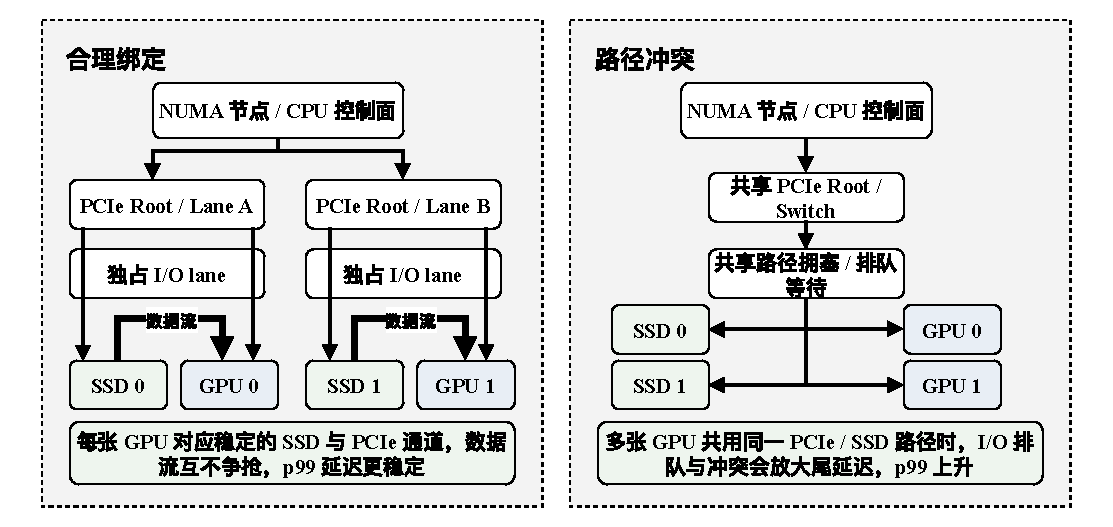
\includegraphics[width=\linewidth]{figures/fig5-3_topology_aware_io_lane.pdf}
  \caption{拓扑感知 I/O 通道示意}
  \label{fig:topology}
\end{figure}

\section{多卡扩展实验与结果分析}

多 GPU 实验沿第三章定义的扩展规模链路逐级组织，并在单卡口径基础上延伸到 100M 样本压力场景；实验围绕索引复制、设备侧归并、主机侧聚合与共享路径冲突（shared-path conflict）四类路径展开，对应配置列入附录B补充表~\ref{tab:multi-gpu-exp-setup}。图~\ref{fig:qps-vs-gpu} 汇总展示索引复制路径的扩展曲线与共享路径下的 p99 延迟变化，图~\ref{fig:latency-quantiles} 展示不同归并路径下的延迟变化，图~\ref{fig:io-lane-impact} 用于比较 I/O 通道配置对扩展性的影响，表~\ref{tab:multi-gpu-summary} 对总体结果进行了汇总。

从结果上看，索引复制方案在 1/2/4 GPU 条件下保持了较为稳定的 QPS 增长和相对平稳的延迟变化，说明在索引可复制的前提下，查询级并行和本地闭环执行更符合本文的吞吐优先目标。与之对应，本地评分 + 设备侧归并和本地评分 + 主机侧聚合的对比主要用于回答兜底路径如何选的问题：两者都建立在索引分片的前提下，但在本文实验口径下，设备侧归并的平均延迟、p99 延迟和 CPU 利用率低于主机侧聚合，说明一旦必须跨卡归并，把局部结果留在设备侧处理更有利于控制路径开销。

另一方面，拓扑感知绑定（Topology-aware binding）与共享路径冲突（Shared-path conflict）的对比表明，即便计算资源足够，当多张 GPU 共享同一 PCIe/SSD 路径时，QPS 仍会明显下降，p99 延迟也会迅速抬升。多 GPU 扩展的实际表现同时受到归并方式和共享路径组织方式的限制。

\begin{figure}[!htbp]
  \centering
  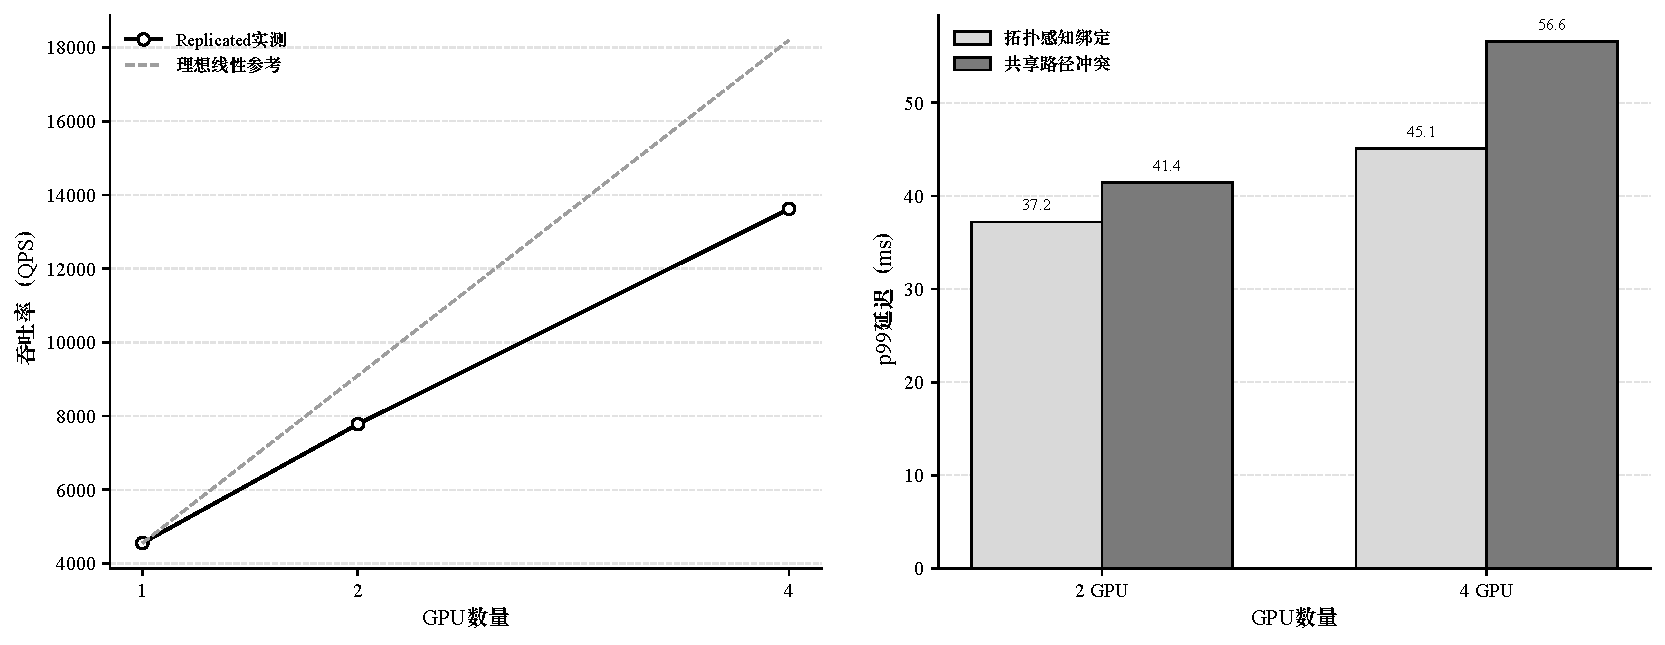
\includegraphics[width=0.95\linewidth]{figures/exp/multigpu_scaling_bottleneck_analysis.pdf}
  \caption{多 GPU 扩展趋势与共享路径瓶颈分析}
  \label{fig:qps-vs-gpu}
\end{figure}

图~\ref{fig:qps-vs-gpu} 左图给出了索引复制路径下 QPS 随 GPU 数量增加的变化，并加入理想线性扩展参考线；该参考线仅由 1 GPU QPS 线性外推得到，是理论参考而非实测结果。实际曲线与理想线性之间存在差距，说明 CPU 控制面调度、查询分发、设备侧资源竞争和 I/O 路径都会削弱扩展效率。右图比较了拓扑感知绑定与共享路径冲突下的 p99 延迟，结果显示共享 PCIe/SSD 路径会放大尾延迟。拓扑感知 I/O 通道绑定因此成为多 GPU 场景下维持稳定扩展的重要条件。对于索引无法完整复制的容量受限场景，仍需结合图~\ref{fig:latency-quantiles} 比较设备侧归并与主机侧聚合：前者把局部结果尽量留在设备侧，后者需要回到主机侧排序与聚合，因此会引入更高的路径开销。

\begin{figure}[!htbp]
  \centering
  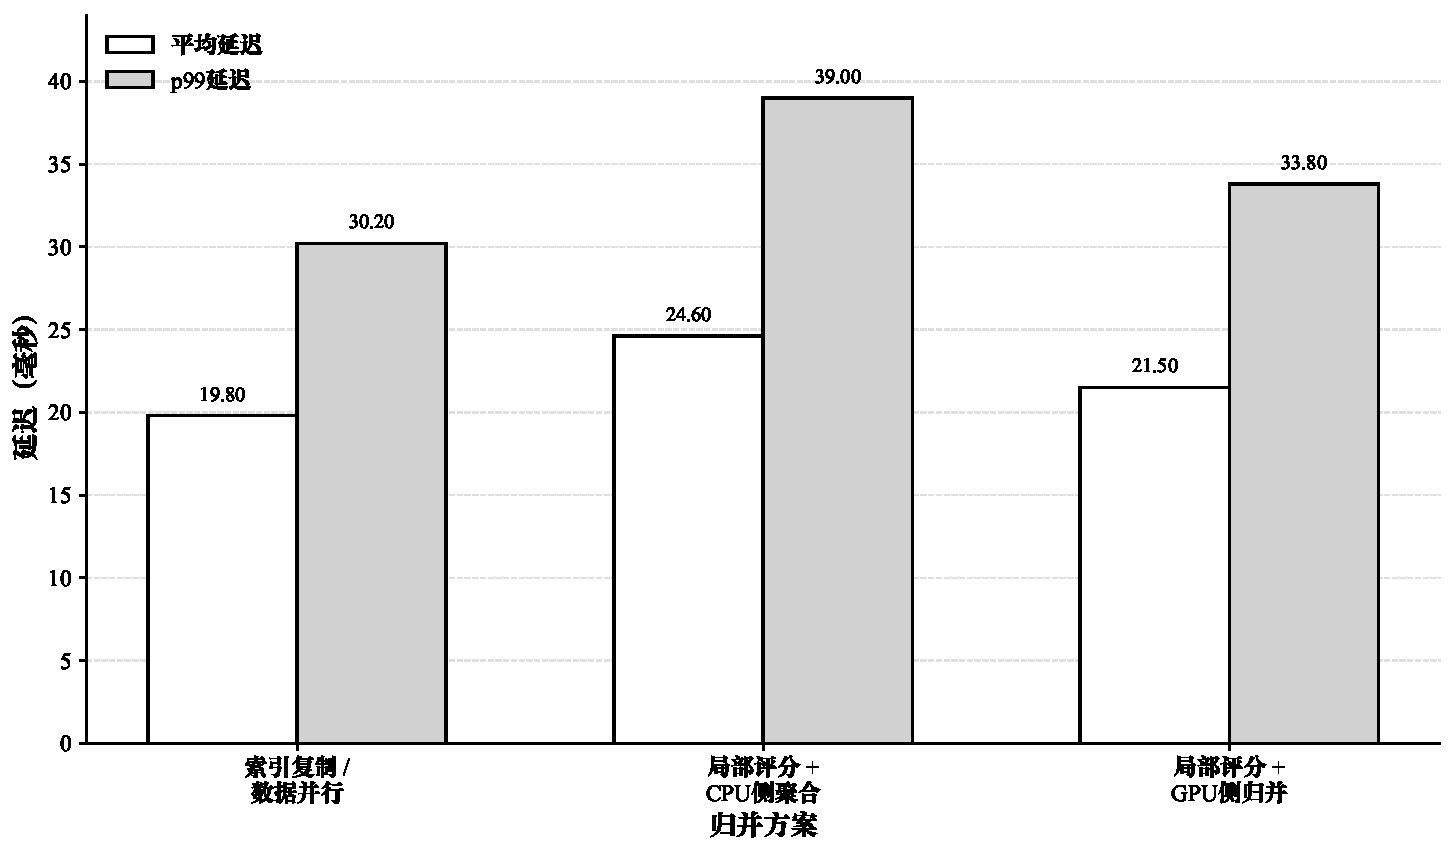
\includegraphics[width=0.84\linewidth]{plot_assets/ch05_latency_merge_compare/fig5_16_latency_merge_compare.pdf}
  \caption{平均延迟与 p99 延迟变化}
  \label{fig:latency-quantiles}
\end{figure}

\begin{figure}[!htbp]
  \centering
  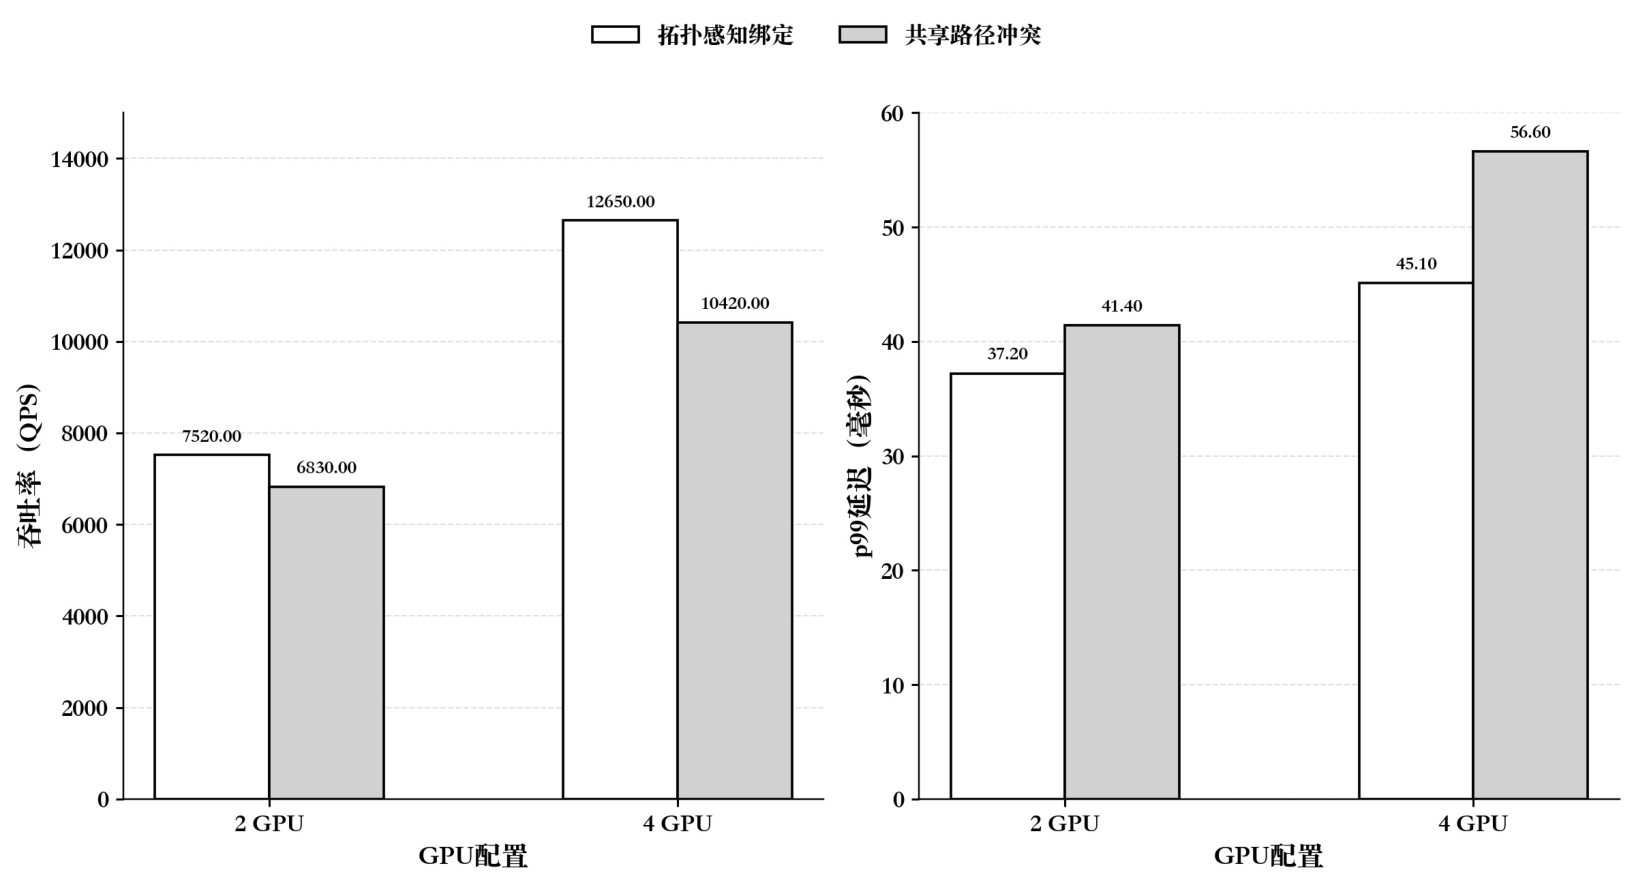
\includegraphics[width=\linewidth]{plot_assets/ch05_io_lane_impact/fig5_18_io_lane_impact.pdf}
  \caption{I/O 通道配置对扩展性的影响}
  \label{fig:io-lane-impact}
\end{figure}

\begin{table}[htbp]
  \caption{多 GPU 扩展结果汇总}
  \label{tab:multi-gpu-summary}
  \centering
  \footnotesize
  \setlength{\tabcolsep}{1.8pt}
  \renewcommand{\arraystretch}{1.18}
  \begin{adjustbox}{max width=\linewidth}
    \begin{tabular}{C{0.75cm}P{2.35cm}C{0.95cm}C{1.35cm}C{1.60cm}C{1.60cm}C{1.45cm}C{1.45cm}}
      \toprule
      GPU数 & 方案 & 数据规模 & QPS & avg\newline latency\newline (ms) & p99\newline latency\newline (ms) & CPU\newline 利用率(\%) & GPU\newline 利用率(\%) \\
      \midrule
      1 & Replicated & 10M & 4550.00 & 22.80 & 34.80 & 47.00 & 63.50 \\
      2 & Replicated & 10M & 7780.00 & 21.00 & 31.90 & 42.00 & 68.80 \\
      4 & Replicated & 10M & 13620.00 & 19.80 & 30.20 & 37.80 & 73.50 \\
      4 & 本地评分 +\newline 设备侧归并 & 100M & 11380.00 & 21.50 & 33.80 & 41.50 & 69.80 \\
      4 & 本地评分 +\newline 主机侧聚合 & 100M & 9580.00 & 24.60 & 39.00 & 48.50 & 62.50 \\
      2 & Topology-aware\newline binding & 100M & 7520.00 & 23.40 & 37.20 & 43.80 & 67.50 \\
      4 & Topology-aware\newline binding & 100M & 12650.00 & 22.10 & 45.10 & 39.80 & 72.20 \\
      2 & Shared-path\newline conflict & 100M & 6830.00 & 25.10 & 41.40 & 45.80 & 61.80 \\
      4 & Shared-path\newline conflict & 100M & 10420.00 & 28.90 & 56.60 & 44.50 & 56.50 \\
      \midrule
      \multicolumn{8}{P{12.2cm}}{\footnotesize 注：结果展示遵循与附录B中补充表~\ref{tab:multi-gpu-exp-setup} 相同的多 GPU 统一规模口径。受版面与结果表达重点限制，表中列出的是 10M 索引复制扩展结果和 100M 压力场景结果，用于回答主方案、兜底路径与共享路径冲突三类设计问题。} \\
      \bottomrule
    \end{tabular}
  \end{adjustbox}
\end{table}

\section{本章小结}

本章把第四章收紧后的单卡 FlashTOD 链路扩展到多 GPU。请求队列、微批形成、任务分发和负载均衡由 CPU 控制面调度；replicated 模式下的索引复制与各卡本地召回---评分闭环属于并行执行。索引无法完整复制时，设备侧归并和 NCCL 通信负责跨卡结果处理，CPU aggregation 作为对照路径；I/O lane 绑定、在途请求控制以及 PCIe/NUMA/SSD 路径选择则属于数据通路优化。这些机制处在不同层次，不能都归为调度。

在表~\ref{tab:multi-gpu-summary} 的 10M replicated 口径下，1、2、4 GPU 的 QPS 分别为 4550、7780 和 13620，4 GPU 达到单卡吞吐的约 2.99 倍。扩展没有保持理想线性，原因来自控制面分发、设备资源竞争以及共享 PCIe/SSD 路径；容量受限时还会增加通信、同步和结果归并。replicated 能复用单卡本地闭环并减少跨卡通信，但每张卡都要保存完整索引，因而提高的是查询吞吐而非单卡索引容量。上述结论只适用于本文单机多 GPU、固定候选预算和既定硬件拓扑。第六章将这些主方案、兜底路径与路径冲突对照放回综合实验口径中考察。
